\chapter{Tracking cancer evolution \textit{in silico} via evolutionary
indices}\label{chapter:trajectories}


\section{Introduction}
A trajectory is a path described by any object (or indeed point) in some space
according to some parameter, usually time.  Intuitively then, an evolutionary
trajectory refers to the changes that a lineage or population undergoes over
time --- the series of genetic, morphological, and behavioral transformations
that occur as organisms evolve and diversify. We are interested in the
evolutionary trajectory of cancers but reliably obtaining time-series data is,
at the time of writing, not feasible at a larger scale. This stems from multiple
issues. Firstly, at time of diagnosis, solid tumours have likely already been
growing for long enough to reach a size visible in standard medical imaging
\cite{patrone_how_2011}. This means that even initial data obtained in the
clinic represents a relatively late stage in the cancer's evolutionary history
most of the time. Secondly, solid tumours are just that --- clumps of cells
organised in some way in space --- meaning that taking a sample from one point
in the tumour is not necessarily representative of the rest of the cell
population. Finally, a biopsy is an invasive procedure which can cause
considerable discomfort to patients, depending on where the tumour is situated.
Therefore, having a reasonable estimate of a tumours evolutionary trajectory
based on the data that is available at time of sequencing would allow for a more
informed treatment strategy. This begs the question --- how can we distinguish
between different ways tumours evolve? Is it necessary to wade through sequences
of genetic data to do so or is it possible to abstract the key properties of a
tumour's evolutionary trajectory into a few numerical summaries? \par In this
chapter, we will examine the utility of two different sets of evolutionary
indices for tracking the evolution of tumours on the example of agent-based
simulations.


\section{Preliminaries}

\subsection{Modes of evolution}
Over the years, there have been a number of different definitions of what a mode
of evolution is. Initially, it was introduced as the term which covers the way
or manner in which a species evolves \cite{eiseley_tempo_1945}. Depending on the
piece of literature, it could also refer to the model used in the study of a
population's evolutionary trajectory \cite{yotoko_does_2011}, or the mechanism
which drives the evolution such as genetic drift \cite{glassman_cancer_1996,
wolf_genome_2013}. This ambiguity of terminology is present in cancer research
as well. In this thesis, I will use the term mode of evolution as originally
defined by \cite{eiseley_tempo_1945}, and used by \cite{davis_tumor_2017,
noble_spatial_2022}. That is, the way in which a tumour evolves (figure
\ref{fig:modes}).

\begin{figure}[h!]
    \centering
    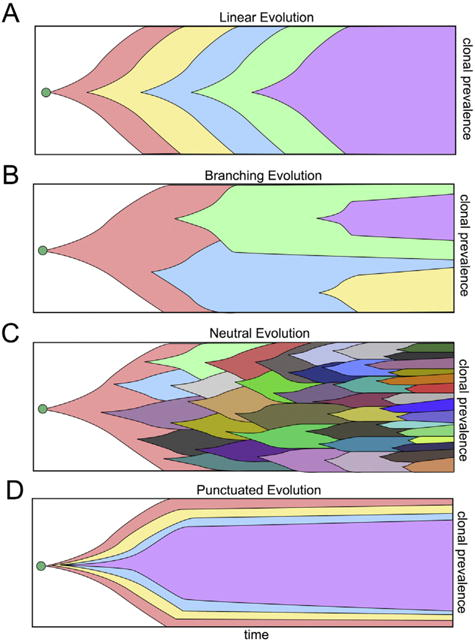
\includegraphics[width=0.85\textwidth]{Chapter_3/figures/modes.jpeg}
    \caption{Four different modes of tumour evolution. \\ Picture adapted from
    \cite{davis_tumor_2017} under a CC BY 4.0 license.}
    \label{fig:modes}
\end{figure}

\subsection{Why even bother with indices?}
Before introducing the sets of indices used to analyse properties of trees, let
us consider a simpler question --- can we map the set of all possible trees to
the set of real numbers? For this purpose we should decide how to define the set
of trees. The number of nodes in a tree is a natural number, $n\in\mathbb{N}$,
as is the number of possible tree topologies for a given $n$. We denote with
$T(n)$ the set of enumerated tree topologies \cite{nakano_tree_2016}. Each node
then has a corresponding size, giving us an $n$-tuple of real numbers
$(\alpha_1, \dots, \alpha_n)\in\mathbb{R}^n$, and each edge (branch) has a
corresponding length or $(l_i, \dots, l_{(n-1)})\in\mathbb{R}^{(n-1)}$. This
means we would need a family of maps

\begin{equation}
    f_n: A(n) \times \mathbb{R}^n \times \mathbb{R}^{n-1} \rightarrow R.
\end{equation}

It would be easy to construct a mapping which would allow us to ``enumerate"
each possible tree with a real number. The problem with this approach, however,
is that it would not be very informative. The real numbers are not ordered in
any way that would allow us to meaningfully compare trees. The lack of
interpretability would render any application of such a mapping useless. This is
where tree shape indices come in as a way to summarise key properties of a tree
in a way that is both interpretable and mathematically sound.

\subsection{A 3-dimensional index space --- trees with uniform branch lengths}

\subsubsection{Shannon diversity}
Shannon entropy is a fundamental concept in information theory, that quantifies
the uncertainty or randomness of a system \cite{shannon_mathematical_1948}. By
considering a system where diversity represents the variety of elements, such as
intra-tumour heterogeneity, we can define the Shannon diversity as the
exponential of the Shannon entropy,

\begin{equation}
    \leftindex[I]^1{D} = \exp\left[\leftindex[I]^1{H}\right] =
    \exp\left[-\sum_{i=1}^N p_i \log p_i\right],
\end{equation}

where $N$ is the total number of categories (or elements, species, etc.), and
$p_i$ the frequency of category $i$. The Shannon diversity was chosen because of
the nice property that it is maximised and equal to the number of categories
when all categories are equally represented, and minimised when only one
category is present. Previous work on a similar topic \cite{noble_spatial_2022}
was based on the Simpson index \cite{simpson_measurement_1949}. However, the
Shannon index was chosen for this work because it is more sensitive to changes
in the frequencies of subclones, better interpretability, and the fact that the
$J^1$ index is based on the Shannon entropy.

\subsubsection{Mean number of drivers per cell --- distance from the root}
Each speciation event in phylogenetics or driver mutation in cancer evolution is
associated with a change in the corresponding tree's topology. To capture the
average number of these events, we use the mean number of drivers per cell. This
is defined as the average of distances from all nodes to the root (with the root
distance from itself defined as $1$) weighted by the frequencies of the
subclones,

\begin{equation}
    n = \sum_{i=1}^N p_i \nu(i),
\end{equation}

where $\nu(i)$ is the root distance of node $i$.

\subsubsection{Balance index}
As discussed in chapter \ref{chapter:trees}, the balance index $J^1$ is a
weighted average of the evenness of the population distribution within a tree.
We use it as the third index in this space.

\subsection{A general set of indices --- any rooted tree}
Expanding upon the $3$-dimensional space defined above, a new comprehensive set
of interpretable robust indices based on Hill numbers was introduced recently
\cite{noble_new_2023}. The authors expanded and improved upon the existing
quantifiers of tree shape properties by deriving methods for trees with
arbitrary node size, node degree, and branch length distributions. The methods
for calculating all of the indices are included as part of an R package
\cite{kimverity_kimverityruiindices_2023}.\par Each generalised index has three
components, depending on which part of the tree it is applied --- the
longitudinal mean, node-wise mean, star mean.

\subsubsection{Richness --- $\leftindex[I]^0{D}$}
Richness in the context of phylogenetics is simply the number of extant species,
i.e. the number of tips in a phylogenetic tree. The generalised richness's
three components are:

\begin{enumerate}
    \item $\leftindex[I]^0{D}_L$ --- the average number of branches across the
        tree;
    \item $\leftindex[I]^0{D}_N$ --- the average effective outdegree, ignoring
        branch sizes;
    \item $\leftindex[I]^0{D}_S$ --- the
        effective number of non-root nodes.
\end{enumerate}

\subsubsection{Diversity --- $\leftindex[I]^q{D}$, $q>0$}
The generalised diversity index represents an extension of the Shannon diversity
index. Its three components are:

\begin{enumerate}
    \item $\leftindex[I]^q{D}_L$ --- the effective number of maximally distant
        nodes (leaves);
    \item $\leftindex[I]^q{D}_N$ --- the average effective outdegree, accounting
        for branch sizes, i.e. bushiness;
    \item $\leftindex[I]^q{D}_S$ --- the effective numbering of branches,
        accounting for branch sizes.
\end{enumerate}

\subsubsection{Evenness --- $\leftindex[I]^q{J}$, $q>0$}
Finally, the extension of the robust universal balance index $J^1$, this set of
indices generalises tree balance in the following way:

\begin{enumerate}
    \item $\leftindex[I]^q{J}_L$ --- evenness of branch sizes across the tree,
        or tree symmetry for leafy and ultrametric trees;
    \item $\leftindex[I]^q{J}_N$ --- tree balance, or evenness of the node size
        distribution;
    \item $\leftindex[I]^q{J}_S$ --- evenness of all branch sizes.
\end{enumerate}


\section{Tree resolution}

I rejected the idea of simply mapping trees to real numbers due to the lack of
interpretability. Tree shape indices are nominally better, as they summarise
properties of a tree, but they may have limitations in the form of a lack of
resolution for certain types of trees. \par
Starting simple, we examine leafy trees with all leaves of equal size in the
$3$-dimensional index space. The first thing to note is that the Shannon
diversity will simply equal the number of leaves in the tree. This already takes
away a degree of freedom. The next thing to consider is the value of $J^1$. If
we limit our search, for now, to perfectly balanced trees, we are left with
symmetric trees on a fixed number of leaves $N$. To make the final index equal
between two trees, they need to have equal average depths of their leaves. As we
are only looking at perfectly symmetric trees, that means that the average depth
will be exactly equal to the individual leaf depths. We can then show the
following
\begin{proposition}
    Let $T$ be a symmetric leafy tree on $N$ leaves with equal leaf sizes. If
    the canonical factorisation of $N$ is
    \begin{equation}
        N = \prod_{i=1}^k \alpha_i^{l_i},
    \end{equation}
    then there are
    \begin{equation}
            \frac{\left(\sum^k_{i=1}l_i\right)!}{\prod_{i=1}^k l_i!}
    \end{equation}
    distinct trees with the same values of $J^1$, $\leftindex[I]^1{D}$, and $n$,
    including $T$.
\end{proposition}
\begin{proof}
    First, the values of indices $J^1$ and $D$ for a symmetric leafy tree with
    $N$ equally-sized leaves are
    \begin{align*}
        J^1 &= 1, \\
        D &= N, \\
        n &= 1 + \sum_{i=1}^k l_i.
    \end{align*}
    The result is then a simple combinatorial problem of placing $n-1$ balls
    ($\alpha_i$'s) into $n-1$ bins, with each $\alpha_i$ repeated $l_i$ times.
    Therefore, the number of distinct trees is
    \begin{equation}
        \frac{\left(\sum^k_{i=1}l_i\right)!}{\prod_{i=1}^k l_i!}.
    \end{equation}
\end{proof}

This case may be interesting mathematically, but is not too relevant for
practical purposes as it is highly unlikely that sequencing data would yield a
perfectly symmetric leafy tree. As the space of trees is so large, there is
little point in performing a grid search, especially when arbitrary node sizes
are considered. In testing, there have been no cases of trees with the same
values of indices, but different topologies. This is a good sign, as it means
that the indices are able to distinguish between different trees. However, the
question remains whether there is a set of indices which can differentiate
between any two trees.

\section{Computational methods}

\subsection{Agent-based modelling framework - \textit{warlock/demon}}
There is no shortage of agent-based models of tumour evolution
\cite{colyer_seven-step_2023}, and the can range from purpose-built complex
frameworks to more stripped-down and abstract ones. Since each model should be
``as simple as possible but no simpler", the appropriate framework for our
purposes must satisfy certain requirements --- flexibility, efficiency, and
reproducibility. The first requirement is deceptively specific. As the main
inspiration behind this work stems from cancer evolution, we want our
simulations to have parameters for controlling aspects of the cell population's
physical properties which would in turn imply a different way in which it
evolves. This would, for example, include spatial arrangement of cells, mutation
rates, migration rates, and selective advantage. Furthermore, while the goal is
to simulate large populations of cells, we also need a large number of
simulations over which we can infer more general deterministic properties.
Stochastic effects could make vastly different evolutionary modes look more
similar than expected in theory. Finally, reproducibility allows us to share
parameters of our models for verification by peers, and possible further
investigation.\\
The agent-based modelling framework we decided to use is \texttt{warlock}
\cite{bak_warlock_2023}, a \texttt{snakemake} wrapper written for \texttt{demon}
\cite{noble_demon_2020}. It satisfies the requirements above, with a few
associated comments. Firstly, it is a flexible agent-based model of tumour
evolution as it does have parameters which control for spatial arrangement,
mutation rates and selective advantage, as well as migration. While it is able
to simulate spatial structure, \texttt{demon} covers at most two spatial
dimensions. This is not an issue since we approximate the cell population to
undergo stochastic isotropic growth, that is the tumour has equal probability of
expanding in all directions in space. This implies approximate spherical
symmetry of simulated solid tumours, which allows us to effectively consider the
two-dimensional simulation as a cross-section of a tumour spheroid. In terms of
efficiency, \texttt{demon} was written mainly in C++, and conceptualised so that
instead of tracking individual cells, it simulates unique cell genotypes on a
two-dimensional grid comprised of demes, or well-mixed patches of cells. The
procedure for simulation cell events is based on the Gillespie algorithm
\cite{gillespie_exact_1977}, and follows the steps of selecting a deme, then
cell type, event type, and finally cell genotype. This approach sacrifices
micro-scale interactions between cells to benefit efficiency and the feasibility
of mathematical analysis of the model using, for example, diffusion
approximations. Finally, all associated code is free and open source (cite
github repos once finished), which allows reproducibility using identical
parameters and random seeds. Parameter values for different batches can be found
in the appendix (ref).


\section{Results}

\subsection{Sensitivity of evolutionary mode to parameter values}

\begin{itemize}
    \item there is clear variance in trajectories within a spatial config but
        less than one might expect for parameters within an order of magnitude
        of each other
    \item all things but spatial config being equal, the trajectories seem to be
        distinct in later stages of evolution
    \item should formalise somehow??
\end{itemize}

\begin{figure} \centering
    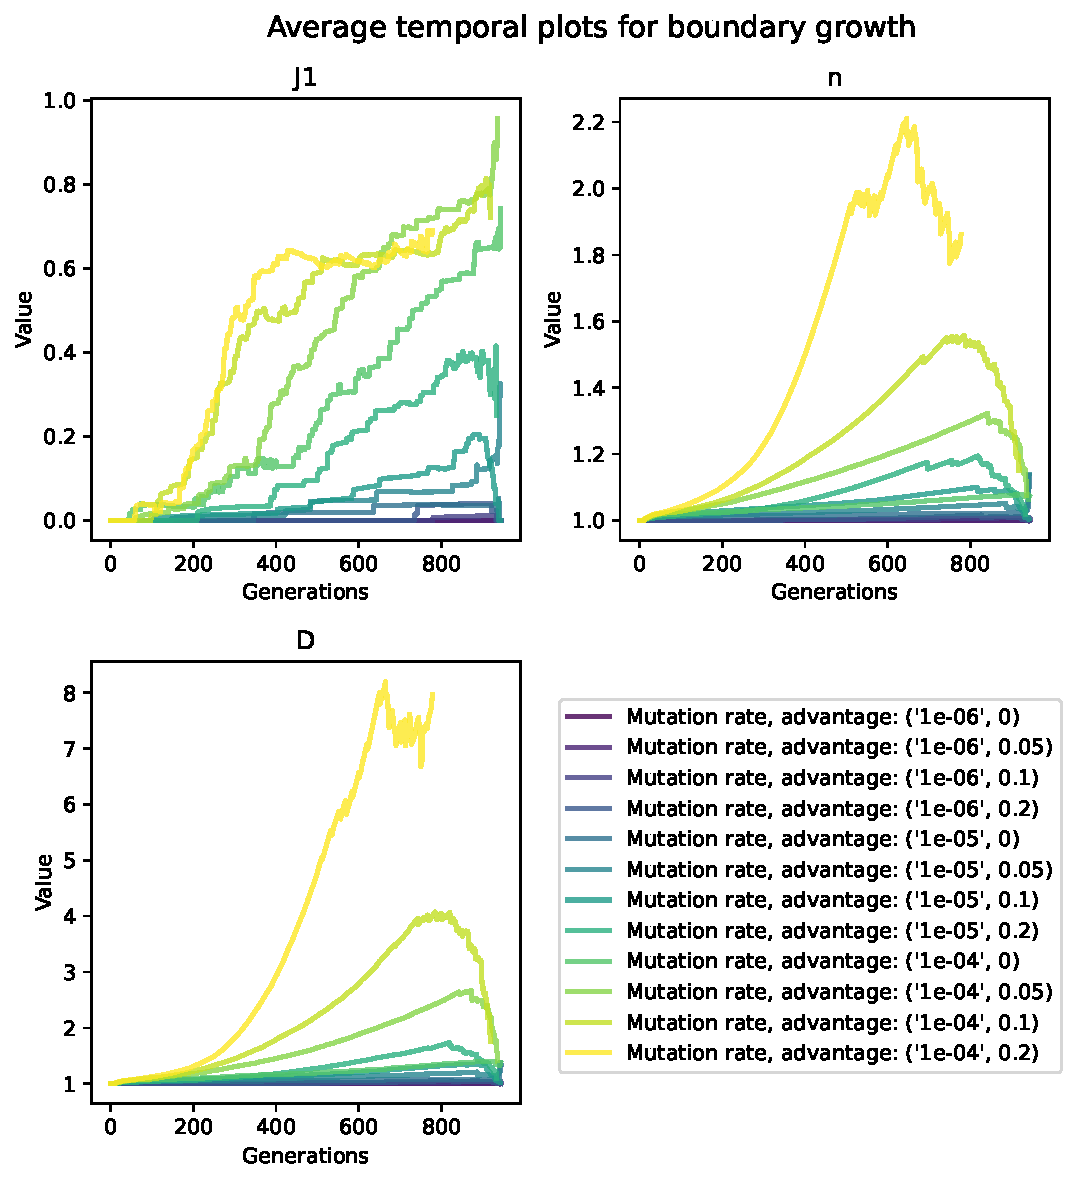
\includegraphics[width=\textwidth]{Chapter_3/figures/boundary-temporal.pdf}
    \caption{Average trajectories of the three indices for different values of
    driver mutation rate and selective advantage for tumours progressing via
    boundary growth.}
    \label{fig:boundary-temporal}
\end{figure}
\begin{figure}
    \centering
    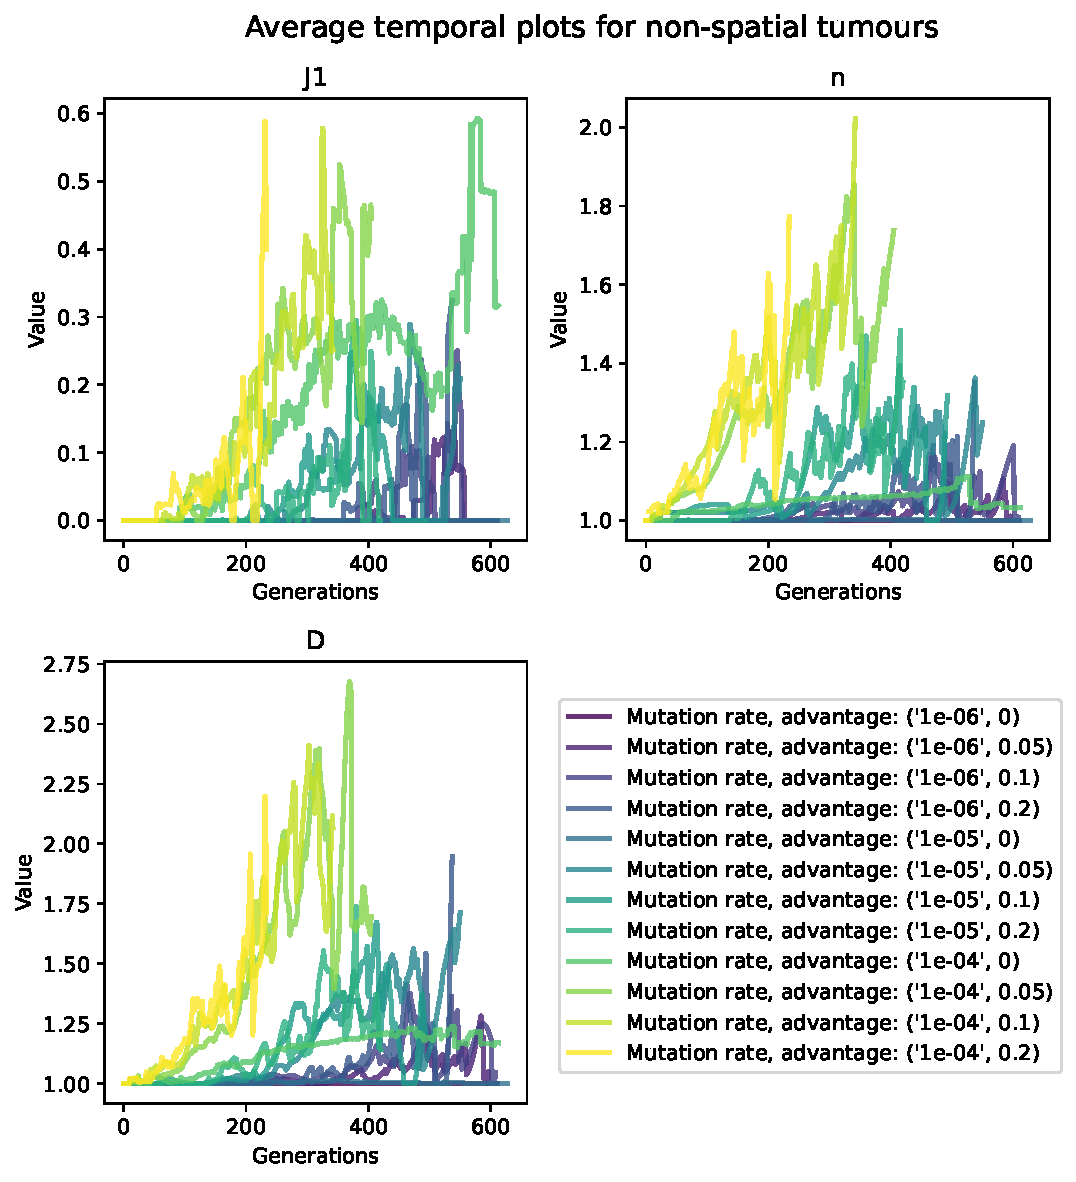
\includegraphics[width=\textwidth]{Chapter_3/figures/non-spatial-temporal.pdf}
    \caption{Average trajectories of the three indices for different values of
    driver mutation rate and selective advantage for well-mixed cancer cell
    populations.}
    \label{fig:non-spatial-temporal}
\end{figure}
\begin{figure}
    \centering
    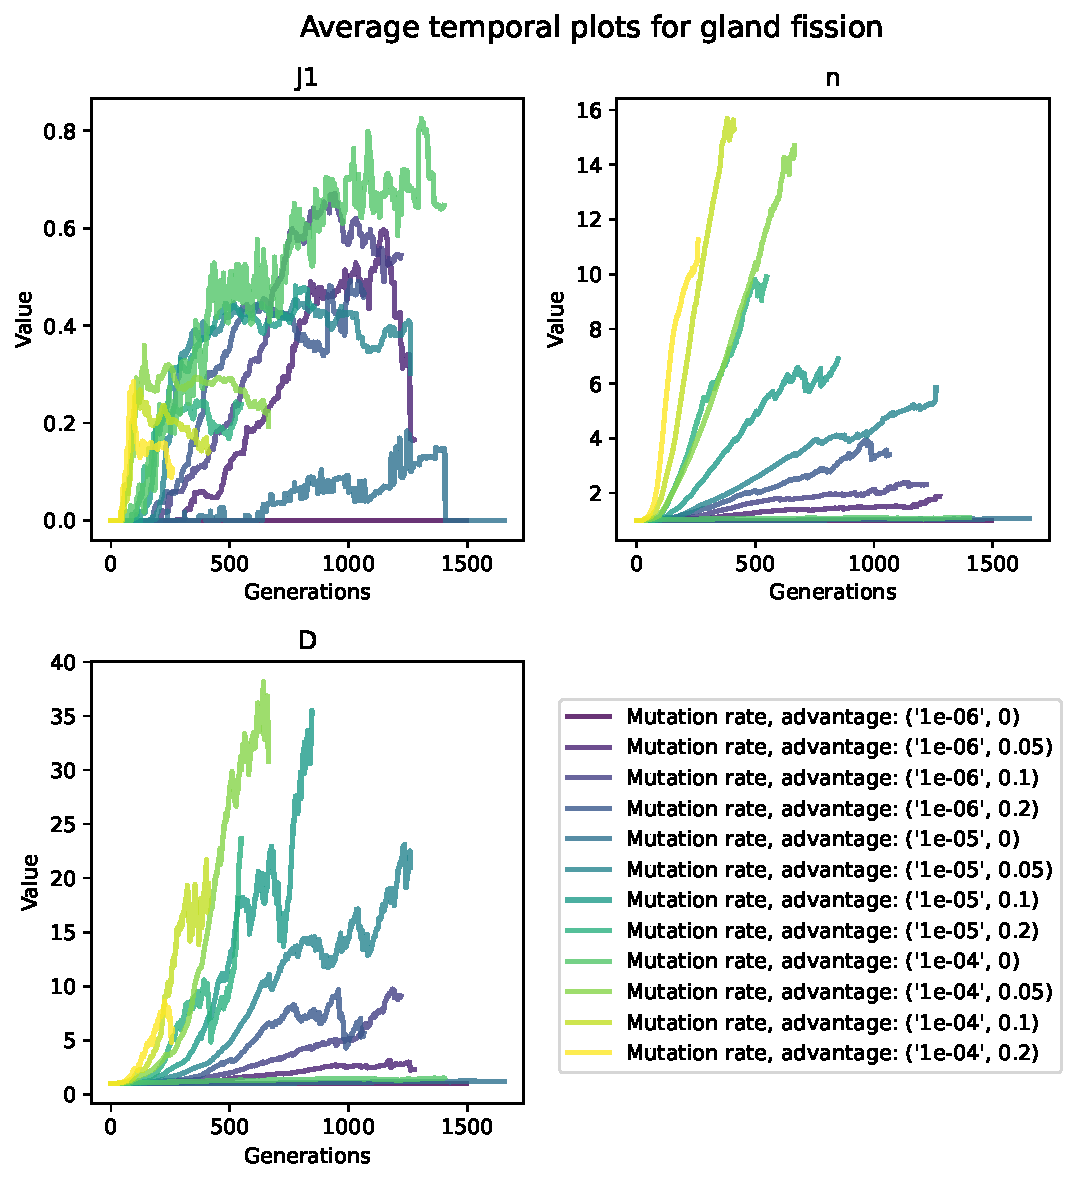
\includegraphics[width=\textwidth]{Chapter_3/figures/gland-temporal.pdf}
    \caption{Average trajectories of the three indices for different values of
    driver mutation rate and selective advantage for gland fission.}
    \label{fig:gland-temporal}
\end{figure}
\begin{figure} \centering
    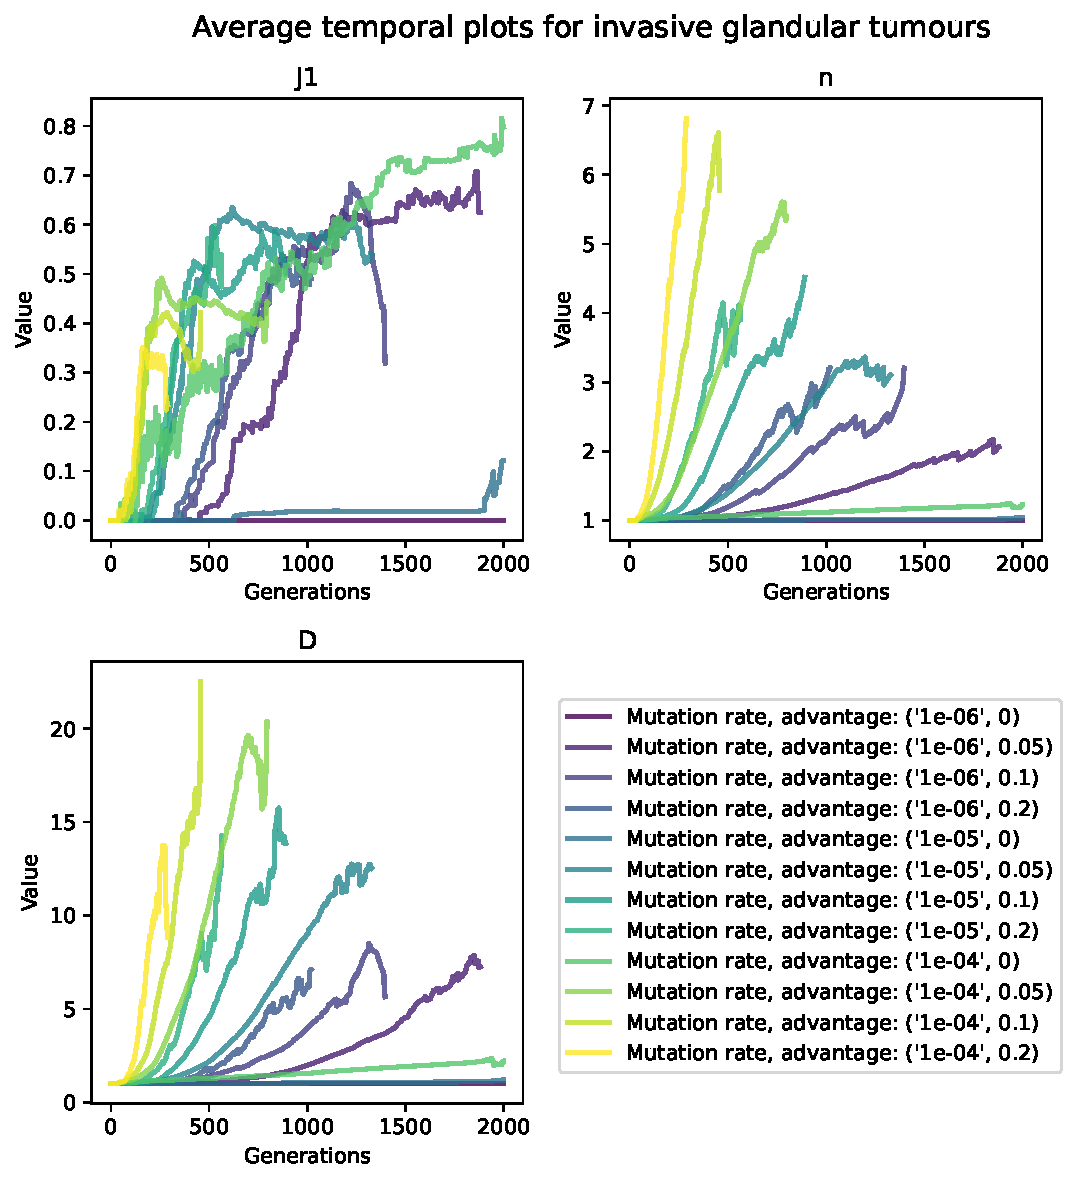
\includegraphics[width=\textwidth]{Chapter_3/figures/inv-gland-temporal.pdf}
    \caption{Average trajectories of the three indices for different values of
    driver mutation rate and selective advantage for invasive glandular
    tumours.}
    \label{fig:inv-gland-temporal}
\end{figure} TO DO: add figures
for index space, add figures to appendix, add expanded index set
figures (both temporal and index space) \begin{figure}
    \centering
    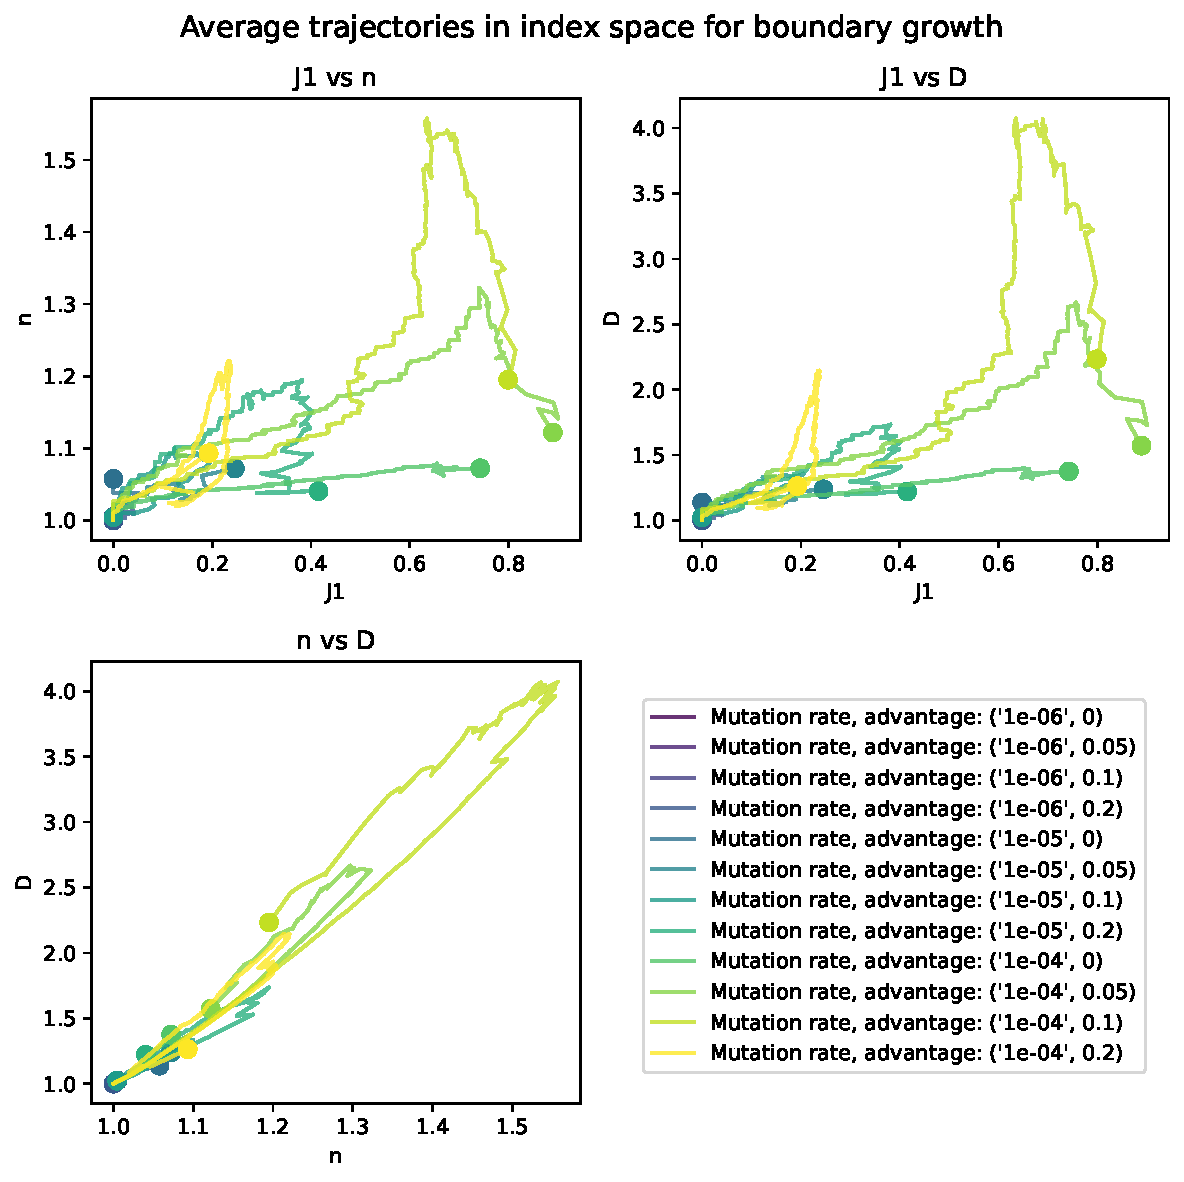
\includegraphics[width=\textwidth]{Chapter_3/figures/indspace-boundary.pdf}
    \caption{Average trajectories in index space for tumours
    progressing via boundary growth.}
    \label{fig:boundary-indspace}
\end{figure}
\begin{figure}
    \centering
    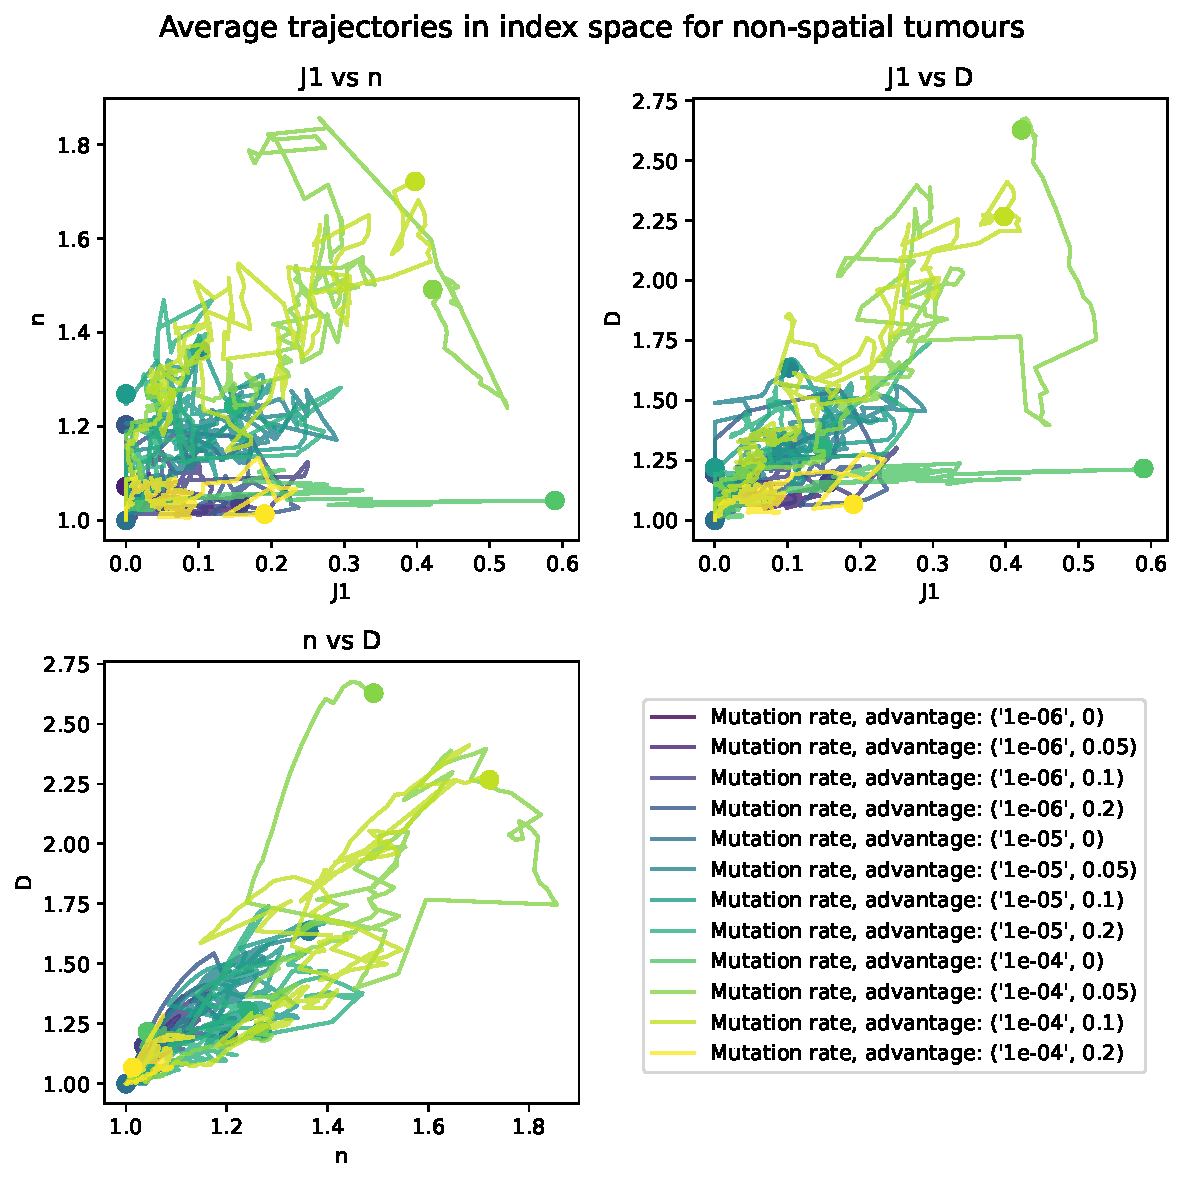
\includegraphics[width=\textwidth]{Chapter_3/figures/indspace-non-spatial.pdf}
    \caption{Average trajectories in index space for well-mixed
    cancer cell populations.}
    \label{fig:non-spatial-indspace}
\end{figure}
\begin{figure} \centering
    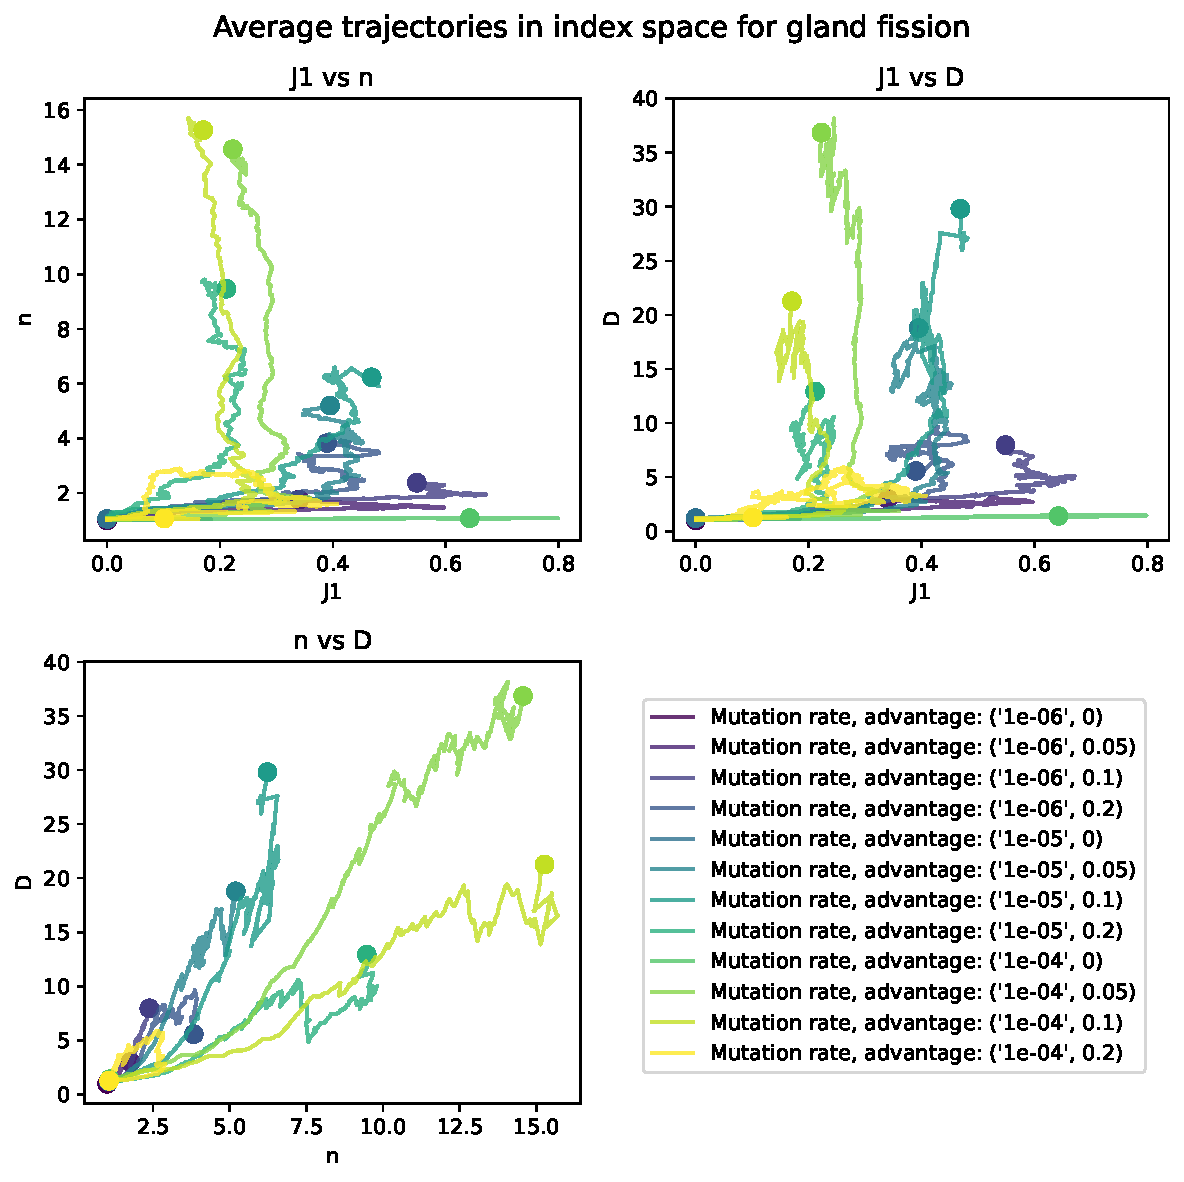
\includegraphics[width=\textwidth]{Chapter_3/figures/indspace-gland.pdf}
    \caption{Average trajectories in index space for tumours
    progressing via gland fission.}
    \label{fig:gland-indspace}
\end{figure}
\begin{figure} \centering
    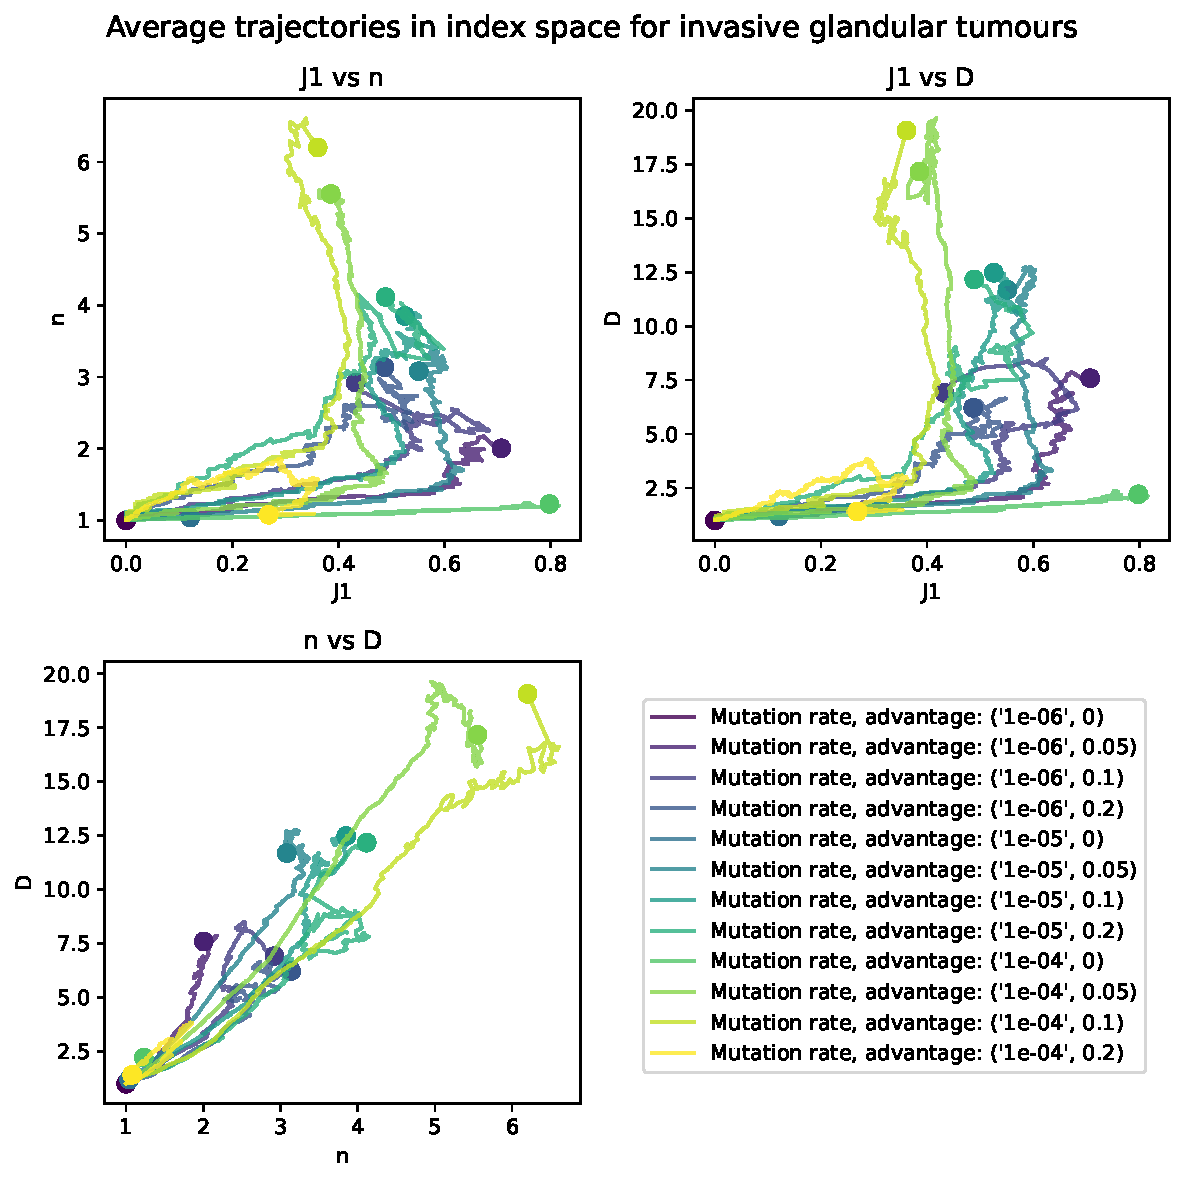
\includegraphics[width=\textwidth]{Chapter_3/figures/indspace-inv-gland.pdf}
    \caption{Average trajectories in index space for invasive
    glandular tumours.}
    \label{fig:inv-gland-indspace}
\end{figure}

% \subsection{Late-stage index-space location implies mode of evolution (?)}
% \begin{itemize} \item focus on the overlaps between (average and overall)
% trajectories of different processes at later stages of tumour growth \item
% consider differences between the base and expanded set of tree indices \item
% based on outputs, come up with a summary statistic which could sort a tumour
% into different based on the end-of-growth state of the tree \end{itemize}


\section{Discussion}

\begin{itemize}
    \item clear differences between different tumour trajectories, but also
        decent amount of variance depending on parameters --- which ones are
        realistic? (need to be inferred from real data)
    \item what are the limitations of the approach? --- clear starting point is
        data availability, but also general inter-patient variation of tumour
        progression
    \item next steps --- further refining of the methods, sourcing and applying
        to more data (Kim's work in progress)
\end{itemize}

